\documentclass[hide notes,intlimits]{beamer}

\mode<presentation>
{
  \usetheme{Singapore}
  \usefonttheme{professionalfonts}
  \setbeamertemplate{blocks}[rounded][shadow=true]
  \setbeamercovered{transparent}
}

% load packages
\usepackage[english]{babel}
\usepackage[latin1]{inputenc}
\usepackage[T1]{fontenc}
\usepackage{lmodern}
\usepackage[multidot]{grffile}
\usepackage{verbatim,empheq}

\usepackage{tikz}
\usetikzlibrary{shapes,arrows,shadows}
\usetikzlibrary{decorations.pathreplacing}

\usepackage{animate}
\usepackage{amsmath,verbatim}

% see http://tex.stackexchange.com/questions/86188/labelling-with-arrows-in-an-automated-way

\newif\ifclipme\clipmetrue
\tikzset{labelstyle/.style={LabelStyle/.append style={#1}},linestyle/.style={LineStyle/.append style={#1}}}
\tikzset{LabelStyle/.initial={},LineStyle/.initial={}}

\newcommand{\mathWithDescription}[4][]{{%
    \tikzset{#1}%
    \tikz[baseline]{
        \node[draw=red,rounded corners,anchor=base] (m#4) {$\displaystyle#2$};
        \ifclipme\begin{pgfinterruptboundingbox}\fi
            \node[above of=m#4,font=\strut, LabelStyle] (l#4) {#3};
            \draw[-,red, LineStyle] (l#4) to (m#4);
        \ifclipme\end{pgfinterruptboundingbox}\fi
    }%
}}

\newcommand{\mathWithDescriptionStarred}[3][]{{%
    \clipmefalse%
    \mathWithDescription[#1]{#2}{#3}{\themathLabelNode}%
}}

\newcounter{mathLabelNode}

\newcommand{\mathLabelBox}[3][]{%
   \stepcounter{mathLabelNode}%
   \mathWithDescription[#1]{#2}{#3}{\themathLabelNode}%
   \vphantom{\mathWithDescriptionStarred[#1]{#2}{#3}{\themathLabelNode}}%
}

\definecolor{dark red}{HTML}{E41A1C}
\definecolor{dark green}{HTML}{4DAF4A}
\definecolor{dark violet}{HTML}{984EA3}
\definecolor{dark blue}{HTML}{084594}
\definecolor{dark orange}{HTML}{FF7F00}
\definecolor{light blue}{HTML}{377EB8}
\definecolor{light red}{HTML}{FB9A99}
\definecolor{light violet}{HTML}{CAB2D6}

\newcommand{\CC}{\mathbb{C}}
\newcommand{\NN}{\mathbb{N}}
\newcommand{\RR}{\mathbb{R}}
\newcommand{\ZZ}{\mathbb{Z}}

\newcommand{\Kcal}{\mathcal{K}}
\newcommand{\Xcal}{\mathcal{X}}

\newcommand{\bF}{\mathbf{F}}
\newcommand{\bQ}{\mathbf{Q}}
\newcommand{\bU}{\mathbf{U}}
\newcommand{\bX}{\mathbf{X}}

\newcommand{\bq}{\mathbf{q}}
\newcommand{\bu}{\mathbf{u}}
\newcommand{\bv}{\mathbf{v}}
\newcommand{\bx}{\mathbf{x}}

\newcommand{\Div}{\nabla\cdot}
\newcommand{\eps}{\epsilon}
\newcommand{\grad}{\nabla}
\newcommand{\lap}{\triangle}
\renewcommand{\bar}{\overline}

\newcommand{\ip}[2]{\ensuremath{\left<#1,#2\right>}}


\newenvironment{transbox}[1][]{%
\begin{tikzpicture}
\node[drop shadow,rounded corners,text width=\textwidth,fill=white, fill opacity=#1,text opacity=1] \bgroup
}{
\egroup;\end{tikzpicture}}


\title[Implicit time-stepping for ice sheets]{Implicit time-stepping for ice sheets}

\author[Bueler]{Ed Bueler}

\institute[UAF]{
  \scriptsize Dept of Mathematics and Statistics and Geophysical Institute \\

  University of Alaska Fairbanks \\
  
  \tiny $^{}$ \\
  \tiny supported by NASA grant \# NNX13AM16G
}

\titlegraphic{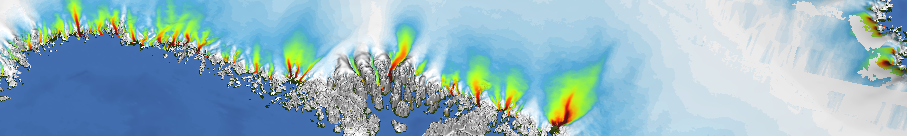
\includegraphics[width=\textwidth]{andycoast.png}}

\setbeamerfont{date}{size=\scriptsize}
\date{}

\AtBeginSection[]
{
  \begin{frame}<beamer>
    \frametitle{Outline}
    %\tableofcontents[currentsection,hideallsubsections]
    \tableofcontents[currentsection]
  \end{frame}
}


\begin{document}

%\graphicspath{{figs/}{../commonfigs/}}
\graphicspath{{../commonfigs/}}

\begin{frame}
\vspace{10mm}
  \titlepage
  \begin{center}
  \tiny SIAM CSE \quad 2 March, 2017
  \end{center}
\end{frame}


\begin{frame}{ice sheet modeling goal: long time, high res runs}

\begin{itemize}
\item \emph{goal}:
\begin{quote}
simulate ice sheets for ice age cycle (\alert{$\sim 10^5$ years}) at resolution (\alert{$\sim 500$ m}) where outlet glaciers, ice streams, and grounding lines are resolved
\end{quote}
\item \emph{main issues}:
    \begin{enumerate}
    \item evolution of ice thickness is diffusive
        \begin{itemize}
        \item[$\circ$] because ice flows downhill
        \end{itemize}
    \item ice margins are steep
    \item bedrock is steep
    \end{enumerate}
\item \emph{natural approach}: implicit time-stepping 
\end{itemize}
\end{frame}


\begin{frame}{ice sheet models}

\begin{itemize}
\item $H=$ thickness, $h=$ surface elevation, $\mathbf{u}=(u,v,w)=$ velocity
\item two models in mind [state variables]:
    \begin{itemize}
    \item[$\circ$] shallow, possibly-hybrid, thickness-based \hfill [$H,(u,v)$]
        \begin{align*}
        H_t + \Div (-D \grad H + \mathbf{u} H) &= m(x,t) && \text{mass conservation} \\
        \mathcal{L}(\mathbf{u},H) &= 0      && \text{shallow stress balance}
        \end{align*}
    \item[$\circ$] Stokes, surface-elevation-based \hfill [$h,(u,v,w)$]
        \begin{align*}
        h_t + \mathbf{u}\big|_h \cdot (h_x,h_y,-1) &= m(x,t) && \text{surface kinematical} \\
        \Div \mathbf{u} &= 0            && \text{incompressibility} \\
        \mathcal{L}(\mathbf{u},h) &= 0  && \text{Stokes stress balance}
        \end{align*}
    \end{itemize}
\item assumptions:
    \begin{itemize}
    \item[$\circ$] conservation of energy ignored
    \item[$\circ$] Eulerian, fixed grid (structured or not)
    \end{itemize}
\end{itemize}
\end{frame}

\begin{frame}{discretize in space}

\begin{itemize}
\item discretize in space and apply implicit time-stepping
    \begin{itemize}
    \item[$\circ$] method of lines = MOL
    \item[$\circ$] (\emph{can you hand the ice sheet problem to an ODE solver?})
    \end{itemize}
\item well-known: MOL for ice sheets is a DAE problem
\begin{align*}
\dot H &= f(H,\mathbf{u},t) && \text{mass conservation} \\
     0 &= g(H,\mathbf{u})   && \text{momentum conservation}
\end{align*}
\vspace{-5mm}
    \begin{itemize}
    \item[$\circ$] (\emph{is implicit time-stepping required for DAEs anyway?})
    \end{itemize}
\item velocity variables exist at positive-thickness locations:
    $$\mathbf{u}_i \text{ exists } \iff H_i > 0$$
\item some ODE solvers can handle \emph{events}:
    \begin{itemize}
    \item[$\circ$] ice disappears during time step:  $H_i(t)>0 \to H_i(t+\Delta t)=0$
    \item[$\circ$] ice appears during time step:  $H_i(t)=0 \to H_i(t+\Delta t)>0$
    \end{itemize}
\end{itemize}
\end{frame}


\begin{frame}{consider: MOL + events}

\begin{center}
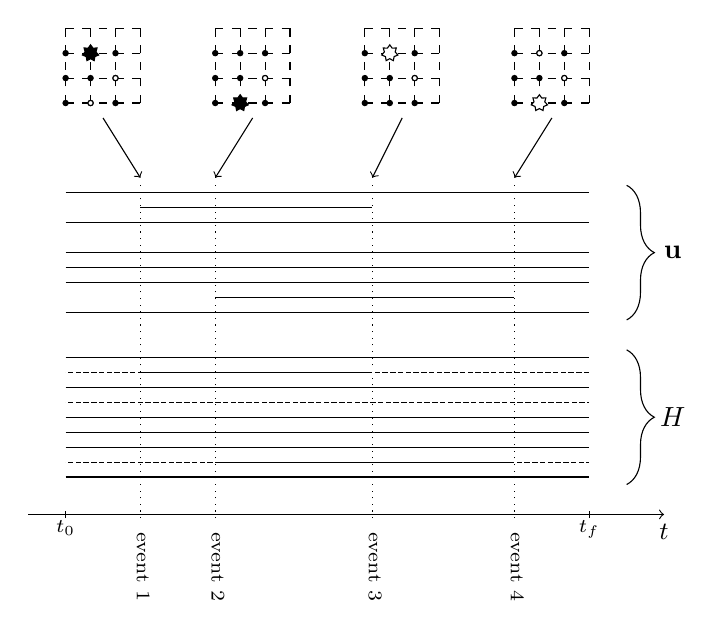
\begin{tikzpicture}[scale=0.95]
  %\draw[->,very thin] (-0.2,0.0) -- (1.2,0.0) node[below] {$x$};
  %\draw[very thin] (0.0,1.0) -- (0.0,0.0) -- (1.0,0.0);
  \pgfmathsetmacro\third{1.0/3.0}
  \pgfmathsetmacro\half{1.0/2.0}
  \pgfmathsetmacro\eps{0.001}

% time axis
  \draw[->,black,thin] (-0.5,-0.5) -- (8.0,-0.5) node[below] {\small $t$};
  \draw (0.0,-0.55) -- (0.0,-0.45) node[below] {\scriptsize $t_0$};
  \draw (7.0,-0.55) -- (7.0,-0.45) node[below] {\scriptsize $t_f$};

% events marked on time axis
  \draw[dotted] (1.0,-0.55) -- (1.0,3.9);
  \node[anchor=north, rotate=-90] at (1.25,-1.2) {\scriptsize event 1};
  \draw[dotted] (2.0,-0.55) -- (2.0,3.9);
  \node[anchor=north, rotate=-90] at (2.25,-1.2) {\scriptsize event 2};
  \draw[dotted] (4.1,-0.55) -- (4.1,3.9);
  \node[anchor=north, rotate=-90] at (4.35,-1.2) {\scriptsize event 3};
  \draw[dotted] (6.0,-0.55) -- (6.0,3.9);
  \node[anchor=north, rotate=-90] at (6.25,-1.2) {\scriptsize event 4};

% time-lines: H
  \foreach \y in {0,...,8} {
      \draw (0.0,\y * 0.2) -- (7.0,\y * 0.2);
  }
  \draw[white,dotted,thick] (0.0,1 * 0.2) -- (2.0,1 * 0.2);     % 1
  \draw[white,dotted,thick] (6.0,1 * 0.2) -- (7.0,1 * 0.2);     % 1
  \draw[white,dotted,thick] (0.0,5 * 0.2) -- (7.0,5 * 0.2);     % 5
  \draw[white,dotted,thick] (0.0,7 * 0.2) -- (1.0,7 * 0.2);     % 7
  \draw[white,dotted,thick] (4.1,7 * 0.2) -- (7.0,7 * 0.2);     % 7
  \draw [decorate,decoration={brace,amplitude=10pt,mirror}] (7.5,-0.1) -- (7.5,1.7) node [black,midway,right,xshift=0.3cm] {$H$};

% time-lines: u
  \pgfmathsetmacro\ushift{2.2}

  \foreach \y in {2,...,4} {
      \draw (0.0,\ushift + \y * 0.2) -- (7.0,\ushift + \y * 0.2);
  }
  \draw (0.0,\ushift + 0 * 0.2) -- (7.0,\ushift + 0 * 0.2);     % 0: full
  \draw (2.0,\ushift + 1 * 0.2) -- (6.0,\ushift + 1 * 0.2);     % 1
                                                                % 5: ice-free
  \draw (0.0,\ushift + 6 * 0.2) -- (7.0,\ushift + 6 * 0.2);     % 6: full
  \draw (1.0,\ushift + 7 * 0.2) -- (4.1,\ushift + 7 * 0.2);     % 7
  \draw (0.0,\ushift + 8 * 0.2) -- (7.0,\ushift + 8 * 0.2);     % 8: full
  \draw [decorate,decoration={brace,amplitude=10pt,mirror}] (7.5,\ushift+-0.1) -- (7.5,\ushift+1.7) node [black,midway,right,xshift=0.35cm] {$\mathbf{u}$};

% grids at events
  \pgfmathsetmacro\gshift{5.0}

  % t = 1.0, node 7 becomes icy
  \draw[xstep=\third,ystep=\third,black,thin,dashed] (0.0-\eps,\gshift+0.0-\eps) grid (1.0,\gshift+1.0);
  \foreach \x in {0,...,2} {
    \foreach \y in {0,...,2} {
        \filldraw (\x * \third,\gshift+\y * \third) circle (1.0pt);
    }
  }
  \node[draw,star,star points=7,fill=black,inner sep=0pt,minimum size=6.0pt] at (\third,\gshift+2 * \third) {};
  \fill[white] (\third,\gshift) circle (1.0pt);            % 1 ice-free
  \draw        (\third,\gshift) circle (1.0pt);
  \fill[white] (2 * \third,\gshift+\third) circle (1.0pt); % 5 ice-free
  \draw[]      (2 * \third,\gshift+\third) circle (1.0pt);
  \draw[->] (\half,\gshift-0.2) -- (1.0,\gshift-1.0);

  % t = 2.0, node 1 becomes icy
  \draw[xstep=\third,ystep=\third,black,thin,dashed] (2.0-\eps,\gshift+0.0-\eps) grid (3.0,\gshift+1.0);
  \foreach \x in {0,...,2} {
    \foreach \y in {0,...,2} {
        \filldraw (2.0 + \x * \third,\gshift+\y * \third) circle (1.0pt);
    }
  }
  \node[draw,star,star points=7,fill=black,inner sep=0pt,minimum size=6.0pt] at (2.0 + \third,\gshift) {};
  \fill[white] (2.0 + 2 * \third,\gshift+\third) circle (1.0pt); % 5 ice-free
  \draw[]      (2.0 + 2 * \third,\gshift+\third) circle (1.0pt);
  \draw[->] (2.0 + \half,\gshift-0.2) -- (2.0,\gshift-1.0);

  % t = 4.1, node 7 becomes ice free
  \draw[xstep=\third,ystep=\third,black,thin,dashed] (4.0-\eps,\gshift+0.0-\eps) grid (5.0,\gshift+1.0);
  \foreach \x in {0,...,2} {
    \foreach \y in {0,...,2} {
        \filldraw (4.0 + \x * \third,\gshift+\y * \third) circle (1.0pt);
    }
  }
  \node[draw,star,star points=7,fill=white,inner sep=0pt,minimum size=6.0pt] at (4.0 + \third,\gshift+2 * \third) {};
  \fill[white] (4.0 + 2 * \third,\gshift+\third) circle (1.0pt); % 5 ice-free
  \draw[]      (4.0 + 2 * \third,\gshift+\third) circle (1.0pt);
  \draw[->] (4.0 + \half,\gshift-0.2) -- (4.1,\gshift-1.0);

  % t = 6.0, node 1 becomes ice free
  \draw[xstep=\third,ystep=\third,black,thin,dashed] (6.0-\eps,\gshift+0.0-\eps) grid (7.0,\gshift+1.0);
  \foreach \x in {0,...,2} {
    \foreach \y in {0,...,2} {
        \filldraw (6.0 + \x * \third,\gshift+\y * \third) circle (1.0pt);
    }
  }
  \node[draw,star,star points=7,fill=white,inner sep=0pt,minimum size=6.0pt] at (6.0 + \third,\gshift) {};
  \fill[white] (6.0 + 2 * \third,\gshift+\third) circle (1.0pt); % 5 ice-free
  \draw[]      (6.0 + 2 * \third,\gshift+\third) circle (1.0pt);
  \fill[white] (6.0 + \third,\gshift+2*\third) circle (1.0pt); % 7 ice-free
  \draw[]      (6.0 + \third,\gshift+2*\third) circle (1.0pt);
  \draw[->] (6.0 + \half,\gshift-0.2) -- (6.0,\gshift-1.0);

\end{tikzpicture}


\end{center}
\end{frame}


\begin{frame}{concerns: MOL + events}

\begin{itemize}
\item \emph{at each event the ice velocity dimension changes}:
    \begin{itemize}
    \item[$\circ$] ``active set'' indexing (e.g.~masks) for velocity variables
    \end{itemize}
\item \emph{events happen all the time on fine grids}:
    \begin{itemize}
    \item[$\circ$] margins of continental-scale ice sheets essentially fractal
    \item[$\circ$] some major climate impacts on scale of a few years (or days)
    \item[$\circ$] need sophisticated ODE event handling
    \end{itemize}
\end{itemize}
\end{frame}




\begin{frame}{weak formulation by variational inequality} 
\begin{itemize}
\item define closed and convex admissible set
  $$\Kcal := \{\eta : \eta^{2p/(p-1)} \in W^{1,p}_0 (\Omega) \,\text{and}\, \eta \ge 0\}$$
over larger domain $\Omega \subset \RR^2$
\item multiply strong form by $\eta-H$ where $\eta\in \Kcal$, and integrate by parts thoughtfully
\end{itemize}
\begin{block}{definition} 
$H \in \Kcal$ solves the \emph{steady shallow ice sheet problem} if
  $$\int_{\Omega}  \Gamma H^{p+1} |\grad s|^{p-2} \grad s \cdot \grad(\eta - H)  
\ge \int_{\Omega} a (\eta - H)$$
for all $\eta \in \Kcal$
\end{block}
\end{frame}


\begin{frame}{ideas contained in weak formulation} 
\begin{itemize}
\item weak form
  $$\int_{\Omega}  \Gamma H^{p+1} |\grad s|^{p-2} \grad s \cdot \grad(\eta - H)  
\ge \int_{\Omega} a (\eta - H)$$
implies strong form
  $$-\Div \left(\Gamma H^{p+1} |\nabla s|^{p-2} \nabla s  \right) =  a$$
where $H>0$
\item weak form also implies: if $H=0$ then $a \le 0$
\item if $b=0$ then the weak form is equivalent to a constrained minimization problem
  \begin{itemize}
  \item[$\circ$] for general bed $b$ this is not so
  \end{itemize}
\end{itemize}
\end{frame}


\begin{frame}{on well-posedness (Jouvet-Bueler 2012)} 
\begin{block}{theorem A.}
if $b=0$ then the variational inequality is equivalent to
  $$\min \, J[u] = \int_{\Omega} \frac{\Gamma}{p} |\grad u|^p - a u$$
over $\eta = u^{(p-1)/(2p)} \in \Kcal$, and this problem is well-posed (existence, uniqueness, stability w.r.t.~data $a$)
\end{block}
\begin{block}{theorem B.}
in general case ($b\ne 0$) there exists a solution
\end{block}
\begin{itemize}
\item proof of B by a fixed-point theorem, of course
\item we really don't know about uniqueness (not just technical)
\end{itemize}
\end{frame}

\end{document}
